\chapter{Magic}
\section{Inroduction}
\section{Which one did you change?}
So we are going to produce a 8x8 grid of elements that we can change to one of two states. It could be a grid of 64 post-it notes of two colours or dots on the screen.
\begin{figure}
    \centering
    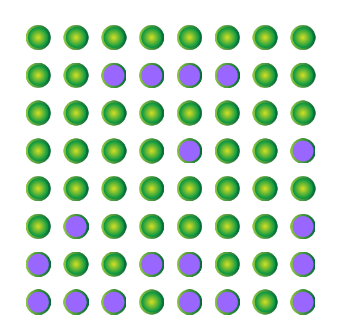
\includegraphics[width=3cm]{chapters/chapterCT1/figures/paritygame.png}
    \caption{Parity Game}
    \label{fig:Parity Game in Scratch}
\end{figure}
\newline
The Scratch code for this can be found at \url{https://scratch.mit.edu/projects/742512502/}
\newline
Now for the first seven rows and first (starting from the left) elements of the grid set the elements to one of the two possible states/colours. 
\begin{figure}
    \centering
    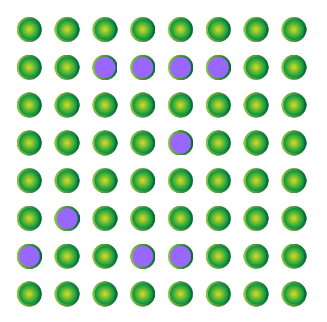
\includegraphics[width=3cm]{chapters/chapterCT1/figures/paritygame2.png}
    \caption{Parity Game starting point}
    \label{fig:Parity Game starting point}
\end{figure}
\newline
So for each row make the number of a particular state be even, so as an example on the fourth row from the top there is only 1 purple dot, so in the last dot on the row we change it from green to purple so there are even number of purple dots on that row. We repeat this for each of the first seven rows. We then do the same for the columns making all the dots in the column be an even number (including the last column) by including a purple dot or not as appropriate.

Now for the trick. Get someone to change one of the dots while the magician looks away. When the magician comes back they are looking for the row and column where the number of particular coloured dot are odd numbered this tells you on which row and column the dot was changed,

This is a concept called Parity where we by making sure all rows and columns have even numbers of particular coloured dots (and you could equally do this with making sure all are odd numbers of particular dots) by adding dots into the extra column and row, we can have built a check for a change.

In Computing we can use this idea to check for an error. Instead of dots, imagine we have 1 or 0 (binary) if we want to transmit 7 bits and we use the 8th bit to make sure the numbers of 1 bits is even when we send the signal (7 bits and the extra bit), if a bit has changed when we recieve it has an odd number of bits, an error has been detected. If we sent the data as 8 blocks with the last 'row' been made up of the bits that make the columns have even number of ones then this will also have change if a single bit has changed but only in the row and column that the changed/error occured so we find the bit and change it back - error correction.

\section{What day of the month is your birthday?}
It is simple but this 'trick' shows the principles of binary and the power of algorithms.I wish I had invented this one.

1.	Say to the participant "If you answer 5 simple questions I can predict which number in the month your birthday is on"

2.	Question 1 "Is the number in Box A?" If the number is the box add 1 otherwise don't add anything. The Magician keeps a running total of the scores.
\newline
\begin{figure}
    \centering
    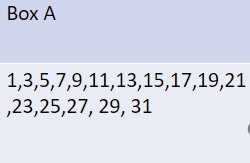
\includegraphics[width=3cm]{chapters/chapterCT1/boxA.png}
    \caption{Box A}
    \label{fig:Box A}
\end{figure}
\newline
3.	Question 2 “Is the number in Box B?" If the number is the box add 2 otherwise don't add anything
\newline
\begin{figure}
    \centering
    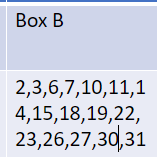
\includegraphics[width=3cm]{chapters/chapterCT1/BoxB.png}
    \caption{Box B}
    \label{fig:Box B}
\end{figure}
\newline
4.	Question 3 “Is the number in Box C?" If the number is the box add 4 otherwise don't add anything
\begin{figure}
    \centering
    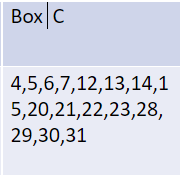
\includegraphics[width=3cm]{chapters/chapterCT1/BoxC.png}
    \caption{Box C}
    \label{fig:Box C}
\end{figure}
5.	Question 4 “Is the number in Box D?" If the number is the box add 8 otherwise don't add anything.
\begin{figure}
    \centering
    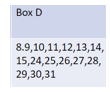
\includegraphics[width=3cm]{chapters/chapterCT1/figures/boxD.png}
    \caption{Box D}
    \label{fig:Box D}
\end{figure}
6.	Question 5 “Is the number in Box E?" If the number is the box add 16 otherwise don't add anything.
\begin{figure}
    \centering
    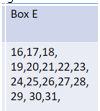
\includegraphics[width=3cm]{chapters/chapterCT1/figures/BoxE.png}
    \caption{Box E}
    \label{fig:Box E}
\end{figure}
7.	Your running total should be the number
What have you done: You have used binary to find the number. For example 27 would be in Box E, Box D , Box B and Box A.which in if we replace the boxes with 1 if the number is in there and 0 if it isn’t; when the boxes are ordered E D C B A we get 11011 which is 27 in decimals. We also have used an algorithm instructions 1 to 6 to get there.
\newline
So lets make it a bit more 'Computer Sciencey,'
Now if we place them into a Table 
\begin{tabular}{lllll} \hline
E & D & C & B & A	 	 \\ \hline
1  & 1  & 0 &  1 & 1\\ \hline

\end{tabular}

Lets instead of A to E we replace the labels with 1, 2,4. 8, 16 each one is the double of the earlier we get:


So 27 is 11011 in binary
\begin{tabular}{lllll} \hline
32 & 16 & 8 & 2 & 1 	 \\ \hline
1  & 1  & 0 &  1 & 1\\ \hline

\end{tabular}
